%!TEX root = thesis.tex

\chapter{Implementation}
\label{ch:Implementation}
The I-POMDP framework was implemented as described in \cite{Butko2010b} with the assumption that the state of the POMDP world does not change within each simulation. This is equivalent to the assumption that when searching for an object in an image, the object does not move.

The implementation was done in MATLAB using object-oriented design, making it easily extensible. It supports parallel execution using MATLAB's Parallel Computing Toolbox\texttrademark{} which allows it to run on multiple cores, or even clusters, to speed up the learning process.

In this chapter the implementation details will be presented and instructions for how to use the framework will be given.

\section{Base Classes}
\label{sec:BaseClasses}
The core of the framework are the two base classes, \texttt{POMDP} and \texttt{Policy}, that contain implementations of methods that are common to different types of POMDPs and policies and define data structures and abstract methods needed for running and training POMDPs.

\subsection{POMDP}
\label{sec:POMDP}
The \texttt{POMDP} base class is a general implementation of a POMDP model. Below are the methods that are implemented in the \texttt{POMDP} base class, which are common to different types of POMDPs.
\begin{description} [style=nextline]
  \item[\texttt{UpdateBelief}]
  This method implements the belief update from equation \eqref{eq:UpdateBeliefFixedTarget}. However, since we can always normalize the belief vector we can instead of equation \eqref{eq:UpdateBeliefFixedTarget} use the proportional belief updates presented in \ref{sec:ProportinalBeliefUpdates}.

  The method depends on the abstract methods \texttt{BeliefDynamics} and \texttt{ObservationLikelihood}. Calling the \texttt{BeliefDynamics} method before updating the agent's belief is necessary to adjust the belief according to the transition model of the POMDP, since the state of the world is not directly observable.

  \item[\texttt{Simulate}]
  This is a method for simulating POMDP episodes for evaluating performance of policies. The method is used by the \texttt{Evaluate} method in the \texttt{POMDP} base class.
\end{description}
The following abstract methods are defined in the \texttt{POMDP} base class.
\begin{description} [style=nextline]
  \item[\texttt{BeliefDynamics}]
  The implementation of this abstract method should apply the system dynamics according to the transition model, introduced in Section \ref{sec:TransitionModel}, to the current belief. This method is called every time the belief is about to be updated.

  In the case of a problem where the state never changes, this method should not change the current belief.

  \item[\texttt{GenerateObservation}]
  The implementation of this abstract method should generate observations according to an observation model, as introduced in Section \ref{sec:ObservationModel}.

  \item[\texttt{ObservationLikelihood}]
  The implementation of this abstract method should calculate the probability of making the current observation, as introduced in Section \ref{sec:ObservationLikelihood}.

  \item[\texttt{Reward}]
  The implementation of this abstract method should calculate the reward according to the reward function, introduced in Section \ref{sec:RewardFunction}.

\end{description}
Additionally, the \texttt{POMDP} base class holds data for the number of actions, number of states, length of observation vectors and the initial belief. These properties should be set in the constructors of the classes that extend the \texttt{POMDP} base class.

\subsection{Policy}
\label{sec:Policy}
The \texttt{Policy} base class is a general implementation of a policy that can be used with a POMDP model. All policies share the same evaluation method implemented in the \texttt{Policy} base class.
\begin{description} [style=nextline]
  \item[\texttt{Evaluate}]
  This is a method for evaluating policies. It runs simulations using the current policy and collects performance data for each simulation.
\end{description}
The following abstract method is defined in the \texttt{Policy} base class.

\begin{description} [style=nextline]
  \item[\texttt{GetAction}]
  This abstract method should contain an implementation of the way the current policy chooses actions.% given the current belief.
\end{description}

\section{Extended Classes}
\label{sec:ExtendedClasses}
In order to make use of the framework, both base classes must be extended by concrete classes that implement the abstract methods defined in the base classes. The framework contains one class that extends the \texttt{POMDP} base class, presented in Section \ref{sec:IPOMDP}, and four classes that extend the \texttt{Policy} base class, presented in Sections \ref{sec:RandomPolicy}, \ref{sec:GreedyPolicy}, \ref{sec:FixateCenterPolicy} and \ref{sec:LogisticPolicy}.

\subsection{IPOMDP}
\label{sec:IPOMDP}
The \texttt{IPOMDP} class extends the \texttt{POMDP} base class and implements its abstract methods. The reward function is information-based and the class is designed for finding objects in an image. This class is essentially an information-driven POMDP and is implemented to be run on the \emph{Where's Waldo?} problem described in \ref{ch:IPOMDP}.

The implementation of each method is described below.

\begin{description} [style=nextline]
  \item[\texttt{Constructor}]
  The purpose of the \texttt{Constructor} method is to initialize values of the POMDP world model. That is, the number of actions available, number of states, length of observation vectors and the initial belief. The observation model parameters are also initialized here.

  \item[\texttt{BeliefDynamics}]
  Since the implementation of the \texttt{IPOMDP} class assumes that the state of the world never changes, i.e. the object in the image does not move, the transition model is according to equation \eqref{eq:IdentityTransitionModel}. In practice this means that the \texttt{BeliefDynamics} method returns the belief state unchanged.

  \item[\texttt{GenerateObservation}]
  The \texttt{GenerateObservation} method contains the implementation of the observation model. The implementation is described in detail in Section \ref{sec:ObservationModelImpl}.

  \item[\texttt{ObservationLikelihood}]
  The implementation of the observation likelihood, described in Section \ref{sec:ObservationLikelihood}, depends on the observation model that is being used. The implementation is described in Section \ref{sec:ObservationLikelihoodImpl}.

  \item[\texttt{Reward}]
  The \texttt{Reward} method is information-based and drives the agent towards minimizing uncertainty about the agent's belief of the world. The implementation is as described in Section \ref{sec:InformationRewards}.
\end{description}

\subsection{RandomPolicy}
\label{sec:RandomPolicy}
The \texttt{RandomPolicy} class implements a policy that selects actions randomly. This class is provided so that other policies can be compared to a random policy.

\subsection{GreedyPolicy}
\label{sec:GreedyPolicy}
The \texttt{GreedyPolicy} class implements a policy that selects the action that corresponds to the state with the highest belief. In other words, given a belief $b_t$ and 
\begin{equation}
  \argmax{i} b_t^i = j
\end{equation}
this policy would select the action $a_t = j$. This class is provided as a benchmark policy that other policies should compete against.

\subsection{FixateCenterPolicy}
\label{sec:FixateCenterPolicy}
The \texttt{FixateCenterPolicy} class implements a policy that always selects the action that corresponds to looking at the center of an image. This class is provided to be able to show how much information can be acquired by only looking at the center of an image.

\subsection{LogisticPolicy}
\label{sec:LogisticPolicy}
The \texttt{LogisticPolicy} class implements a policy that is parameterized as a logistic function. The way this logistic function selects actions is described in Section \ref{sec:LogisticPolicies}. This policy is a stochastic policy.

The class also implements a training method, \texttt{Train}, for learning policies using the policy gradient method described in \ref{sec:PolicyGradient}. Section \ref{sec:PolicyTraining} explains how to to train a policy using the training method.

\section{Class Diagrams}
This section contains diagrams of the base classes and their extended implementations introduced in the previous sections, Sections \ref{sec:BaseClasses} and \ref{sec:ExtendedClasses}.

\subsection{POMDP Classes}
The following diagram shows the relationship between the \texttt{IPOMDP} class described in Section \ref{sec:IPOMDP} and the \texttt{POMDP} base class described in Section \ref{sec:POMDP}.

\begin{figure}[tb]
  \centering
  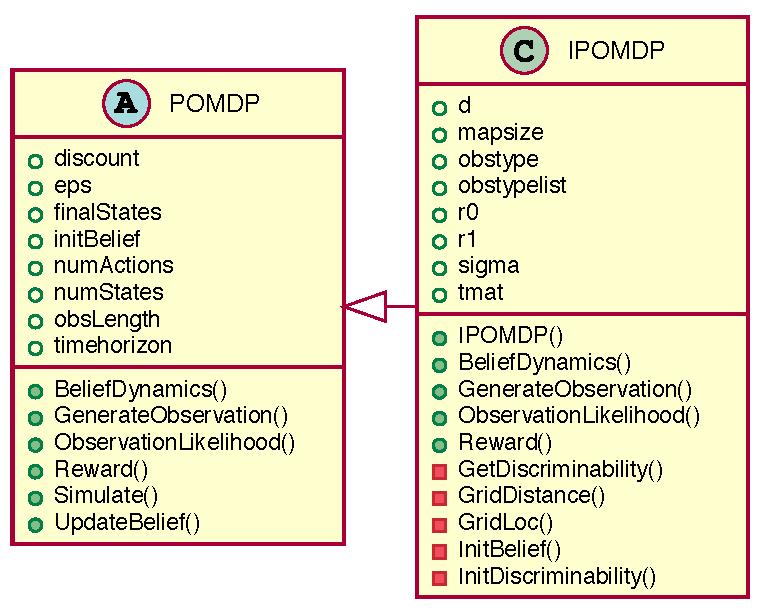
\includegraphics[width=0.6\textwidth]{figures/POMDPClasses}
  \caption{This class diagram shows the relationship between the \texttt{IPOMDP} class and the \texttt{POMDP} base class.}
  \label{fig:POMDPClasses}
\end{figure}

\FloatBarrier

\subsection{Policy Classes}
The following diagram shows the relationships between the different policy classes, described in Sections \ref{sec:RandomPolicy}, \ref{sec:GreedyPolicy}, \ref{sec:FixateCenterPolicy} and \ref{sec:LogisticPolicy}, and the \texttt{Policy} base class described in Section \ref{sec:Policy}.

\begin{figure}[tb]
  \centering
  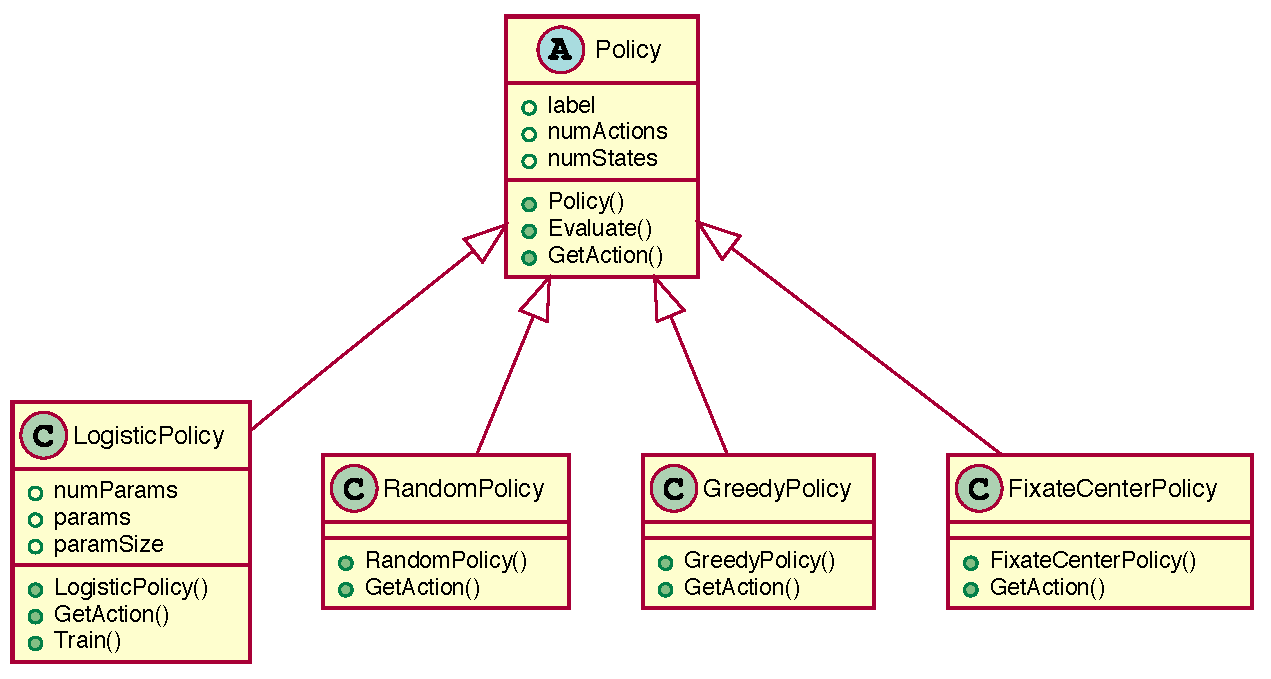
\includegraphics[width=1\textwidth]{figures/PolicyClasses}
  \caption{This class diagram shows the relationships between the different policy classes and the \texttt{Policy} base class.}
  \label{fig:PolicyClasses}
\end{figure}

\section{Training a Policy}
\label{sec:PolicyTraining}
Training a policy requires calling the \texttt{Train} method in the \texttt{LogisticPolicy} class with a set of parameters. The necessary parameters and their purpose are listed below.
\begin{description} [style=nextline]
  \item[\texttt{POMDP}]
  An instance of a class derived from the \texttt{POMDP} base class that implements all of its abstract methods, for example the \texttt{IPOMDP} class. This is where the simulation of each episode takes place.

  \item[\texttt{Epochs}]
  The number of training iterations. The policy parameters are updated after each iteration.

  The default value is $2000$.

  \item[\texttt{Episodes}]
  The number of belief trajectories that are sampled for each epoch. The policy gradient is calculated in each episode and the average policy gradient over all episodes is used after each epoch to update the policy parameters.

  The default value is $150$.

  \item[\texttt{T}]
  The time horizon of the POMDP, i.e. the number of time steps to run in each episode.

  The default value is equal to the number of states.

  \item[\texttt{Eta}]
  The learning rate.

  The default value is $0.02$.

  \item[\texttt{Beta}]
  The Bias-variance trade-off parameter. The value of \texttt{Beta} should be between $0$ and $1$, where $\texttt{Beta} = 0$ minimizes the effect of variance and $\texttt{Beta} = 1$ is unbiased.

  The default value is $0.75$.
\end{description}
After training the method will return the initial policy with updated policy parameters.

\section{Performance Improvements}
Programs written in MATLAB are not always computationally efficient and training a policy with 4,900 iterations and 150 episodes in each iteration is a time-consuming task. Therefore measures were taken to reduce the time it takes to train a policy.

\subsection{Computational Complexity}
The most time consuming part of the policy training is calculating the policy gradient. The policy gradient is calculated in every time step so the total number of times it is calculated during training is given by
\begin{equation}
  \texttt{T} \times \texttt{Episodes} \times \texttt{Epochs}
\end{equation}
The policy gradient algorithm depends on the number of states and actions. If the number of states is equal to the number of actions, i.e. $n = |\mathcal{S}| = |\mathcal{A}|$, then its time complexity is
\begin{equation}
  T(n) = \BigO{n^2}
\end{equation}
For this reason it is important that the policy gradient algorithm is implemented with efficiency in mind.

\subsection{MEX File}
To speed up training, the policy gradient algorithm was implemented in C code and plugged into the MATLAB code by compiling it to a MEX file (MATLAB executable). The C implementation of the policy gradient algorithm can be viewed in Appendix \ref{app:GradientCImplementation}.

\subsection{Parallel Execution}
Another speed improvement was made by making the policy training method support parallel execution. This was done using MATLAB's Parallel Computing Toolbox\texttrademark{} by making the sampling of belief trajectories (i.e. each episode) run in a parallel for-loop instead of a normal one. This allows more than one iterations of the for-loop to run simultaneously resulting in faster execution, given that there are more than one cores available.

\subsection{Results}
The results of the performance improvements can be seen in Figure \ref{fig:PerformanceImprovement}.

\begin{figure}[!htp]
  \centering
  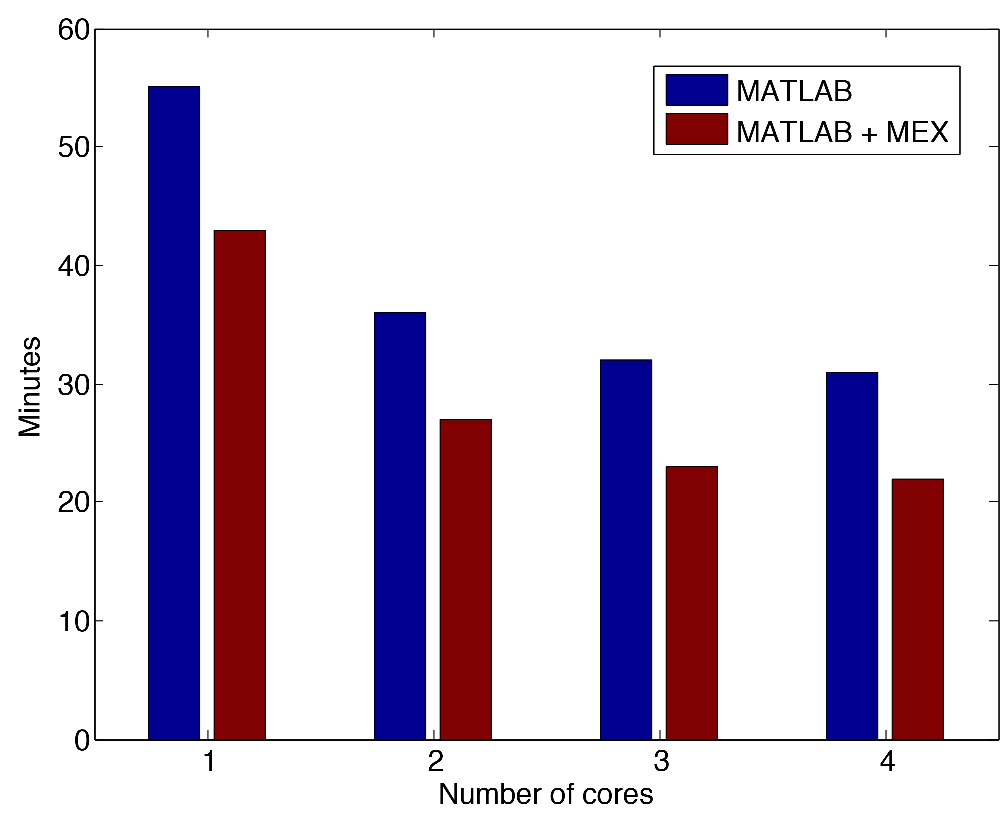
\includegraphics[width=0.5\textwidth]{figures/performance_improvement}
  \caption{Running times of policy training with 2,000 iterations and 150 episodes per iteration, 49 states ($7 \times 7$ grid) and time horizon $T$ equal to the number of states, 49.}
  \label{fig:PerformanceImprovement}
\end{figure}
